\msusection{Application Details} \label{sec:advanced}
The following section details of the operation of YCweather.  This section is meant to aid researchers at the Subzero Science and Engineering Research Facility maintain and update the software.  YCweather was written with MATLAB version 7.9.0.529 (R2009b).  If you are using a newer version of MATLAB for editting YCweather the MATLAB run time component must be updated on all machines attempting to execute YCweather (see Section \ref{sec:compile} for additional details).

\msusubsection{Basic YCweather Operations}
The executable version of YCweather relies on four primary files that must be located in the same location: \texttt{YCweather.exe}, \texttt{YCmain.exe}, \texttt{default.mat}, and \texttt{version.txt}.  \texttt{YCweather.exe} is a wrapper program that keeps the main program \texttt{YCmain.exe} current based on the installed version (\texttt{version.txt}) and the available version on the YCweather website (Section \ref{sec:compile}).  \texttt{YCmain.exe} may be executed without \texttt{YCweather.exe}, but will never update in this case.  The source code for \texttt{YCweather.exe} and \texttt{YCmain.exe} are MATLAB m-files \texttt{YCweather.m} and \texttt{MAIN.m}, respectively.  \texttt{YCweather.m} will not operate correctly via the m-file; \texttt{MAIN.m} may be run via MATLAB if desired.

When \texttt{YCmain.exe} begins it opens the \texttt{default.mat} workspace file, which must be located in the same directory.  If this file does not exist or it is the first execution of YCweather this file is created.  The workspace file includes the location of the database directory that contains all the weather data, daily logs, and image files.  This directory may be located anywhere on the machine as long as the workspace file points to the correct location (see Sections \ref{sec:pref}).  However, when the \texttt{default.mat} workspace file is created the location is initially set as the \q{database} folder in the same directory as the YCweather executables.

When \texttt{YCmain.exe} (\texttt{MAIN.m}) begins operation, after opening the workspace file (\texttt{default.mat}), it attempts to download the latest weather data.  As mentioned in Section \ref{sec:data} this option may be turned off.  The installation package, Section \ref{sec:compile}, includes the latest data from the current season.  Thus, an Internet connection is not required to run YCweather initially, but only to keep the program and data current.  Lastly, \texttt{YCmain.m} initializes by applying the \texttt{default.mat} workspace file (\texttt{callback\_readWS.m}), prior to this the only two parameters in the workspace file where utilized: the database location and the auto update trigger.

At this point, the YCweather is ready for manipulation by the user and the program has opened all available data into the internal data structures.

\msusubsection{Database Directory}\label{sec:database}
The database directory must be organized in a specific fashion for YCweather to operate correctly, most of this organization is handled automatically.  The directory tree for the YCweather database is shown in Figure \ref{fig:filestructure}.  The first level of folders in the database directory are for each season of data, these exact folder names show up in the Program Control window in the Season/Folder pop-up menu.  The initialization of the pop-up menu occurs when a workspace file is opened, the source code being \texttt{callback\_readWS.m}.

When the user selects the season via the pop-up menu YCweather accesses this folder, inside of which the *.yc format files (see Section \ref{sec:formatfile}) for all weather stations are stored.  These format files contain, among other things, an abbreviated station name.  This name is used in the internal data structure of YCweather as well as for creating the next level of folders.

As described in Section \ref{sec:data}, YCweather acts as an archiving application for daily logs and images.  The daily logs, images, or image reference files are contained in folders that exist within the station folders.  The folders are named according the aforementioned abbreviated station name.  Within each of these folders two additional folders exist: DailyLogs and Images.  These folders, as the names suggest, store the archived daily logs and image files.  The station folders and sub-folders are created automatically by YCweather when the user adds a daily log or image (see Section \ref{sec:add}).

The DailyLog folder contains text files that store the daily log information, each log must me named as \texttt{mm-dd-yy.txt}.  The Images folder contains folders named as \texttt{mm-dd-yy}.  Within each folder the images are stored, the names are irrelevant, but the files should be stored only in recognized formats, see MATLAB's help on \q{imread}.  This directory may also contain a \texttt{images.txt} file which contains a list of image files elsewhere on the computer that have been associated with the station and data by the user, see Section \ref{sec:add}.

\begin{figure}[h]\centering
	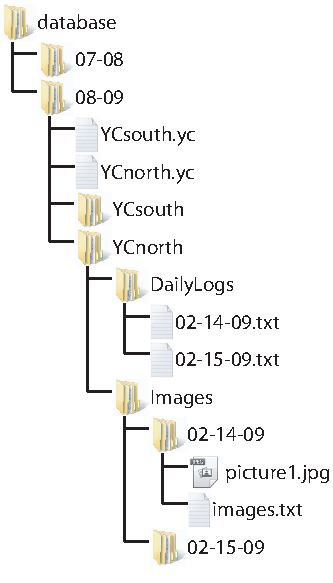
\includegraphics[]{\YCfiles figures/filestructure.pdf}
	\caption{Example of file structure of the database directory used by YCweather.}
	\label{fig:filestructure}
\end{figure}

\msusubsection{Weather Station Format Files (*.yc)}\label{sec:formatfile}
YCweather basis it's entire operation on format files, which are simply text files with a *.yc extension.  An example, format file is include in Figure \ref{fig:formatfile}.  These files communicate to YCweather the necessary information regarding the weather data files.  The weather data files may be any comma delimited text file completely composed of columnar numeric entries.

\begin{figure}[h]\centering
	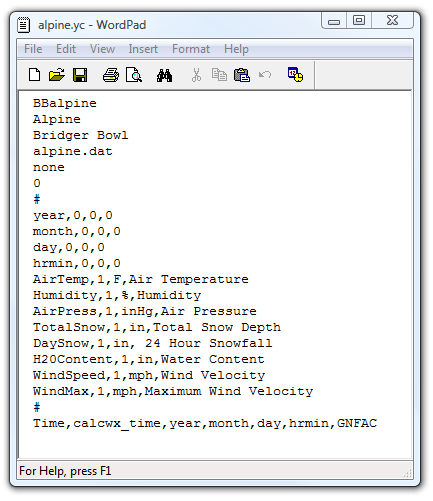
\includegraphics[width=0.55\linewidth]{\YCfiles figures/formatfile}
	\caption{Example format file utilzed by YCweather.}
	\label{fig:formatfile}
\end{figure}

Format files are composed of three parts, with the parts being separated by \# sign.  The first portion consists of six lines that detail various parts of the data file.  Part two details each column of data present in the data file.  Finally, part three contains custom functions utilized for making calculations.

\msusubsubsection{Part One: Data File Details}
The following list is a line-by-line description of the six components required in the first portion of the *.yc format files.

\begin{enumerate}
	\nitem{Station ID:} The station id must be a single text string that uniquely identifies the weather station associated with this data file.  This ID must conform to MATLAB's variable naming convention, see MATLAB's help file on \q{Naming Variables}.
	\nitem{Station name:} This string identifies the weather station and will appear next to the toggle button within the Station Panel in the Program Control window.
	\nitem{Station location:} This value is a text string that identifies the location of the weather station, this name will appear in the Station Panel in the Program Control Window.
	\nitem{Path to data file:} The path to the data file must be any valid complete or relative path and filename that references the data file associated with this format file.  In the example file, Figure \ref{fig:formatfile}, the file \texttt{alpine.dat} must then exist in the same directory as the *.yc format file.
	\nitem{Array ID:} This value is useful for weather files that are composed of multiple data arrays such as created via Campbell Scientific dataloggers.  In many cases data files of this type contain a identifier at the beginning of a row identify the type of data.  For example, a row beginning with 60 may represent hourly data and those starting with 24 may indicate daily data.  Thus, if the Array ID is 60 in the *.yc format file then only the data marked with this ID would be included for this station in YCweather.  Another *.yc file would need to be established to gather the data from the other array.  Figure \ref{fig:formatfile2} includes the Array ID feature.  In Array ID is present in the file, \texttt{none} should be entered in this location.
	\nitem{Thermocouple ID:} This identifier indicates if a thermocouple array within the snowpack exists.  If this data does not exist then \texttt{0} (zero) should be entered.  For stations with snowpack temperature arrays this ID should correspond the the variable ID's defined in part two of the *.yc file, as discussed below and shown in Figure \ref{fig:formatfile2}.  The variable ID also must contain a numeric portion that indicates the location of each thermocouple in the snowpack.  For example, the thermocouples shown in Figure \ref{fig:formatfile2} are space at 2 cm intervals.
\end{enumerate}

\begin{figure}[!ht]\centering
	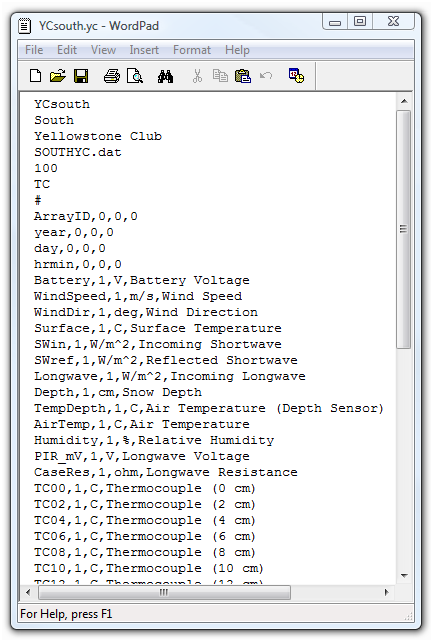
\includegraphics[width=0.55\linewidth]{\YCfiles figures/formatfile2}
	\caption{Example format file utilized by YCweather that includes the thermocouple ID for plotting temperature profile data (this is not a complete file).}
	\label{fig:formatfile2}
\end{figure}

\msusubsubsection{Part Two: Weather Variables}
Part two details the weather variables, there should be one row for each column that exists in the corresponding data file.  Each row in this section has four comma separated values, as detailed below.

\begin{enumerate}
	\nitem{Variable Name:} The first value is a single string of text that uniquely defines the variable from others in the format file. This name must conform to MATLAB's variable naming convention, see MATLAB's help file on \q{Naming Variables}.
	\nitem{Inclusion Trigger:} This value indicates to YCweather if the corresponding column of data should be listed as a selectable option in the program.  Entries may be 0 or 1, where 0 excludes the data.
	\nitem{Units:} The third entry communicates the units of the data; this value must conform to the units specified in the \texttt{units.txt} file as detailed in Section \ref{sec:units}.  The units can be in either English or metric units, but must be included in the aforementioned file.
	\nitem{Legend Label:} The last value is a string describing the weather data that is inserted into the legends of YCweather graphs.
\end{enumerate}

\msusubsubsection{Part Three: Custom Functions}
This section allows for calculation to be done on the weather variables listed above in Part Two.  One function that is a critical component of YCweather will be used here as an example, the \texttt{calcwx\_time.m} function. \textbf{YCweather requires that a variable named \texttt{Time} be present and contain the time stamps for the weather data in MATLAB's serial format.} The \texttt{calcwx\_time.m} function performs this operation. For information on this format see MATLAB's help on \q{Types of Date Formats}.  

Taking a step back, the function \texttt{read\_dat.m} is responsible for reading the format *.yc files, this function outputs the weather data into a structure that is used by YCweather; \texttt{read\_dat.m} also implements the custom functions listed in the *.yc format files.

When the custom function are called from \texttt{read\_dat.m} they are implemented as follows within MATLAB, using \texttt{calcwx\_time.m} as an example.
\begin{Verbatim}[fontsize=\small , frame=single, label=MATLAB]
>> Time = calcwx_time(d,'year','month','day','hrmin','GNFAC');
\end{Verbatim}

Comparing this functional operation to the row of inputs in the format file in Figure \ref{fig:formatfile} shows that the first entry in the format *.yc file is the output variable (\texttt{Time}), the next value is the function name (\texttt{calcwx\_time}), and the remaining items are string input into the custom function.  The input variable d is the data structure used for storing the weather data and is automatically inputed into the custom function in \texttt{read\_dat.m}.  This data structure contains all the data present in the weather data file, as listed in Part Two.  Hence, the function \texttt{calcwx\_time.m} uses the input strings (\texttt{'year','month'}, etc.) to compute the new Time variable with the appropriate time format required by YCweather.  So, each custom function essentially creates another weather variable for use by YCweather.

The custom functions were setup to allow YCweather to be expandable by the user to perform calculations on the weather data.  To best understand the custom functions, it is best to examine the source code, specifically section five of \texttt{read\_dat.m} and any of the existing custom functions: \texttt{calcwx\_time.m, calcwx\_flux.m}, and \texttt{calcwx\_labLW.m}.

\msusubsection{Variable Units}\label{sec:units}
As mentioned in Section \ref{sec:formatfile}, the format files require that the units for each weather variable be defined.  The units prescribed in the format file must be present in the \texttt{units.txt} file, which is read by the \texttt{getunit.m} function.  The \texttt{units.txt} defines the units via text abbreviations (e.g., \texttt{'kPa'} for pressure) both in Metric and English, the conversion factor between the units, and the appropriate axis labels for use in YCweather generated graphs. The function \texttt{getunit.m} is utilized for extracting the various unit related information in various portions of YCweather.  Both the function \texttt{getunit.m} and text file \texttt{units.txt} were designed to allow for additional units to be added, which should only require adding a row to the text file. 

The \texttt{units.txt} file should be composed of rows containing the following comma separated information: 1) the Metric abbreviation, 2) the English abbreviation, 3) text describing the unit, 4) the Metric abbreviation written in \LaTeX ~math format, 5) the English abbreviation written in \LaTeX ~math format, 6) the Metric unit written as \TeX, 7) the English unit written as \TeX, 7), and finally 8) the conversion multiplier from English to Metric.  Figure \ref{fig:units} contains a portion of the \texttt{units.txt} file, refer to the file itself for additional examples as well as additional information regarding the format.  Note, the \# is the comment character within the file.

\begin{figure}[!ht]\centering
	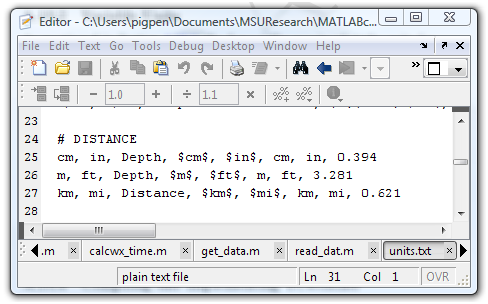
\includegraphics[width=0.55\linewidth]{\YCfiles figures/units.png}
	\caption{Example entries for prescribing units within the \texttt{units.txt} file, which is utilized by the \texttt{getunit.m} function.}
	\label{fig:units}
\end{figure}

\msusubsection{Compiling and Implementing YCweather}\label{sec:compile}
The information in this section details the process for building a YCweather executable file from the source code via MATLAB's compiler. Note, that if a 32-bit version of MATLAB is being used the compiler is included, otherwise a compiler must be installed (see \href{http://www.mathworks.com/support/compilers/R2010a/}{\nolinkurl{www.mathworks.com/support/compilers/R2010a/}}). The \texttt{mbuild -setup} function in MATLAB is used to setup your compiler initially.  

If any changes are made to the source code of YCweather the following information will make the updates available to all users running YCweather. The function \texttt{YCbuild.m} acts to automate the process of compiling YCweather into executable form as well as post the updated to the web folder.  The function requires two outside programs, WinSCP\footnote{\href{http://winscp.net}{WinSCP: winscp.net}} and InstallJammer\footnote{\href{http://www.installjammer.com/}{InstallJammer: www.installjammer.com}}.

After changing the source code, implement the the following code from the MATLAB command-line: \texttt{>>YCbuild('build',0.5)}, where the second input is the new version number.  When this command executes the version is updated, YCweather.exe and YCmean.exe are complied, YCmain.zip is packaged, the latest weather data from the current season is prepared, and the installer is compiled (YCinstaller.exe).  All of these files are placed in the \texttt{release} directory, which are exactly the files need on the YCweather website.  Before compiling a new version, the version number in the \texttt{MAIN.m} functions should be updated.

This process relies on three files.  First, the two project files: YCweather.prj and YCmain.prj.  These files were created with MATLAB's \texttt{deploytool} and dictate how YCweather.exe and YCmain.exe are compilied.  If any additional m-files are added to YCweather then these files will needed to be added to the list of files in the YCmain.prj file.  The third file, is the InstallJammer installation file, YCinstaller.mpi, which is stored in the YCinstallerFiles directory.

Once YCweather is complied it must also be uploaded to the website so that the changes will be made available to all users of the program.  This is done by executing the following: \texttt{>>YCbuild('web')}.  This removes the old files from the web and adds the new via WinSCP; access to the appropriate account on the MSU Department of Civil Engineering server is required. 

\msusubsection{Website and Online Weather Database}\label{sec:web}
The YCweather website, \href{http://www.coe.montana.edu/ce/subzero/snow/}{www.coe.montana.edu/ce/subzero/snow}, is hosted by the MSU College of Engineering and contains the installation files YCweather and the files for automatically updating YCweather.  These files are automatically generated during the compilation and posting process described in Section \ref{sec:compile}.

YCweather also relies on an ftp accessible database hosted by the College of Engineering, which contains the weather files database directories that are accessed by YCweather for keeping the weather data up to date.  The MATLAB program \texttt{GNAFC.m} located on the server is executed hourly to keep the weather data current via CRONTAB.
